\section{Introducción}

Cuando un usuario accede a un sitio web o intenta transmitir información de un punto a otro por medio de la web, el mismo en general se abstrae de todos los mecanismos necesarios requeridos para esta transmisión. Dada la gran cantidad y heterogeneidad del hardware subyacente, en lo comienzos de la web se empezaron a diseñar distintos tipos de protocolos de comunicación para lograr unificar todos estos dispositivos en una red capaz de transmitir información desde cualquier punto a otro de forma relativamente confiable.

Hoy en día, el protocolo dominante para la transmisión de datos por la red es el IP (Internet Protocol). Creado por Vint Cerf y Bob Kahn en 1974, el protocolo IP esta diseñado para ser utilizado en redes de conmutación de paquetes y no esta orientado a conexión. Esto significa que al enviar un archivo, el mismo es fragmentado en paquetes que no necesariamente siguen la misma ruta en la red. Además, al no ser un protocolo orientado a conexión, no hay garantías de que los paquetes lleguen a destino dado que no hay ningún tipo de protocolo de handshake entre origen y destino.

En relación al modelo OSI, el protocolo IP pertenece a la capa de internet. Existen muchos otros protocolos que han sido construidos sobre el protocolo IP con el objetivo de proveer otro tipo de garantías y funcionalidades, entre los mas conocidos se encuentran el protocolo TCP (Transmission Control Protocol) y el UDP (User Datagram Protocol). Estos protocolos pertenecen a la capa de interconexión.

En el presente trabajo utilizaremos el protocolo ICMP (Internet Control Message Protocol), el cual esta especificado en el RFC 792 \cite{RFC}, con el objetivo de analizar las diferentes trazas y el RTT (round trip time) al momento de conectarse a un sitio web. Una traza se define como la sucesión de dispositivos de red que son recorridos, ya sean puentes, routers o gateways, al momento de transmitir información en la red. El protocolo ICMP esta implementado sobre IP, aunque se considera que el mismo no pertenece a la capa de interconexión a diferencia de TCP y UDP. Esto se debe a que su principal propósito no es intercambiar datos entre sistemas, si no que en general se utilizan para enviar mensajes de error entre dispositivos de red, con la excepción de su uso en herramientas como ping y traceroute.

\subsection{Traceroute}

La herramienta traceroute, desarrollada inicialmente por Van Jacobson en 1988, es una herramienta sumamente útil de diagnostico de red para buscar una aproximación de la traza de conexión y encontrar el RTT a cada hop (o salto) en la traza. Como ya hemos mencionado, esta herramienta utiliza el protocolo ICMP. A continuación discutiremos la estructura de los paquetes IP/ICMP para luego explicar como se hace efectivamente para identificar los diferentes hops. Luego discutiremos que potenciales problemas puede tener esta herramienta.

\subsection{Header IP}

Como ya hemos mencionado, el protocolo ICMP esta implementado sobre IP. A continuación mostramos la estructura del header de un paquete IPv4. Todo lo que mencionaremos sigue siendo valido para IPv6.

\begin{figure}[H]
  \vspace{2em}
  \begin{center}
    \begin{bytefield}[bitwidth=1.1em]{32}
      \bitheader{0-31} \\
      \bitbox{4}{Version} & \bitbox{4}{IHL}  & \bitbox{6}{DSCP} & \bitbox{2}{ECN} & \bitbox{16}{Total Length}  \\
      \bitbox{16}{Identification} & \bitbox{3}{Flags}  & \bitbox{13}{Fragment Offset}  \\
      \bitbox{8}{Time To Live} & \bitbox{8}{Protocol}  & \bitbox{16}{Header Checksum}  \\
      \bitbox{32}{\emph{Source IP Address}} \\
      \bitbox{32}{\emph{Destination IP Address}} \\
      \bitbox{32}{\emph{Options (if IHL $>$ 5)}} \\
    \end{bytefield}
  \end{center}
  \caption{Header IPv4}
  \label{fig:ipv4-packet}
\end{figure}

Como podemos observador, el header de un paquete IPv4 tiene 24 bytes. En este momento, el campo que mas nos interesa es Time To Live (TTL). Como lo dice su nombre, este campo fue pensado para imponer un limite de tiempo a la vida del paquete en la red. Si no llegaba el paquete antes de ese tiempo, el mismo era descartado por el correspondiente hop. Sin embargo, en la practica esto se implemento como un limite a la cantidad de hops que un paquete podía recorrer. Esto se ve en los headers de los paquetes IPv6, donde el campo fue renombrado como Hop Limit.

\subsection{Header ICMP}

En los paquetes IP/ICMP, al header de IP se le suma el header de ICMP. El mismo tiene la siguiente estructura:

\begin{figure}[H]
  \vspace{2em}
  \begin{center}
    \begin{bytefield}[bitwidth=1.1em]{32}
      \bitheader{0-31} \\
      \bitbox{8}{Type} & \bitbox{8}{Code} & \bitbox{16}{Header Checksum} \\
      \bitbox{16}{Identifier} & \bitbox{16}{Sequence Number} \\
      \bitbox{32}{\emph{Datos}}
    \end{bytefield}
  \end{center}
  \caption{Header ICMP}
  \label{fig:icmp-header}
\end{figure}

El protocolo ICMP es parte del Internet Protocol Suite, especificado en RFC 792. Este header de 12 bytes se ubica luego del header de IP, teniendo un tamaño de header total de 36 bytes. La especificación explica en detalle como se utiliza el protocolo normalmente. Lo bueno de este protocolo es que si en algún momento header de IP llega a un $ttl = 0$, el hop correspondiente devolverá un mensaje de error al cliente de origen. En unos momentos veremos porque esto es sumamente útil.

En nuestro caso, los siguientes casos de type seran los mas relevantes:

\begin{itemize}
	\item Type 0 – Echo Reply
	\item Type 3 - Destination Unreachable
	\item Type 8 – Echo Request
	\item Type 11 – Time Exceeded
\end{itemize}

En principio, implementaremos nuestra propia herramienta traceroute utilizando paquetes ICMP. Para ello, enviaremos un Echo Request al URL (Uniform Resource Locator) al que queremos acceder y encontrar la traza utilizando el campo TTL del header IP.

Si el paquete llega al destino, el servidor nos enviara un paquete ICMP con el type Echo Reply. Para poder encontrar los diferentes hops en la traza, utilizaremos el parámetro Time To Live del header IP, inicializándolo en 1 y luego aumentándolo hasta que nos respondan con un Echo Reply. Es decir, si estamos interesados en identificar el hop $i$ de la traza, tendremos que settear el parametro $TTL = i$ y luego enviar el request.

Cuando TTL llega a 0, si el hop implementa ICMP, el mismo nos devolverá un reply de tipo Time Exceeded, incluyendo en la sección de datos del paquete ICMP el header IP y los primeros 8 bytes de del datagrama de datos original que enviamos. Si el hop se encuentra bajo algún tipo de congestión, es posible que el mismo descarte nuestro paquete para priorizar los de protocolos como TCP o UDP. Esto por supuesto depende de la implementación del dispositivo de red correspondiente.

Notar que no necesariamente el servidor estara disponible o aceptara paquetes ICMP, por lo que tendremos que poner un limite a la cantidad de hops que buscaremos. Caso contrario iteraríamos hasta llegar al limite dado por los 8 bytes del campo TTL, lo cual no tiene sentido practico. Este procedimiento se puede ver un poco mejor en la siguiente imagen:

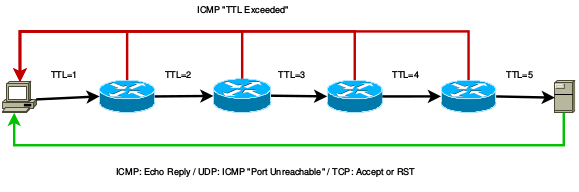
\includegraphics[width=\textwidth,keepaspectratio]{images/traceroute_typical}

Para implementar esta herramienta utilizaremos Python, con la libreria Scapy. Esta librería nos permite formar paquetes ICMP y luego hacer los respectivos requests.

\subsection{Resolución DNS}

Al hacer un request, en general nos abstraemos de la direccion IP y lo hacemos a un URL. Este URL se debe resolver a una dirección IP mediante un request a un DNS (Domain Name System) con el formato especificado en el RFC 1035 \footnote{RFC 1035: \url{https://www.ietf.org/rfc/rfc1035.txt}}. Por lo tanto, correr dos veces la herramienta no nos garantizara que hagamos el request a un mismo IP, dado que un sitio puede tener varios IPs asignados. Esto pasa normalmente con google.com. A su vez, en el ejemplo ilustrativo consideramos una topología de red sumamente simple. Dado que las topologías tienden a ser sumamente complejas, esto lleva a que al hacer el traceroute se puedan presentar una serie de problemas que deben ser tenidos en cuenta.

\subsection{Anomalidades en traceroutes}

A continuación veremos las potenciales problemáticas de hacer un traceroute utilizando paquetes ICMP. En general las mismas surgen debido a la complejidad innata de las topologías de red. Las mismas en general se pueden agrupar en los siguientes tipos:

\begin{enumerate}
	\item Missing hops
	\item Missing destination
	\item False RRTs
	\item Missing links
	\item Loops and Circles
	\item Diamonds
\end{enumerate}

Estos tipos están explicados en detalle en el paper de Jobst \cite{jobst2012traceroute}.